%%%%%%%%%%%%%%%%%%%%%%%%%%%%%%%%%%%%%%%%%%%%%%%%%%%%%%%%%%%%%%%%%%%%%
% LaTeX Template: Project Titlepage Modified (v 0.1) by rcx
%
% Original Source: http://www.howtotex.com
% Date: February 2014
% 
% This is a title page template which be used for articles & reports.
% 
% This is the modified version of the original Latex template from
% aforementioned website.
% 
%%%%%%%%%%%%%%%%%%%%%%%%%%%%%%%%%%%%%%%%%%%%%%%%%%%%%%%%%%%%%%%%%%%%%%

\documentclass[12pt]{report}
\usepackage[a4paper]{geometry}
\usepackage[myheadings]{fullpage}
\usepackage{fancyhdr}
\usepackage{lastpage}
\usepackage{graphicx, wrapfig, subcaption, setspace, booktabs}
\usepackage[T1]{fontenc}
\usepackage[font=small, labelfont=bf]{caption}
\usepackage{fourier}
\usepackage[protrusion=true, expansion=true]{microtype}
\usepackage[english]{babel}
\usepackage{sectsty}
\usepackage{url, lipsum}
\usepackage{listings}
\usepackage{color}
\usepackage{hyperref}
\usepackage{graphicx}
\graphicspath{ {images/} }

\newcommand{\HRule}[1]{\rule{\linewidth}{#1}}
\onehalfspacing
\setcounter{tocdepth}{5}
\setcounter{secnumdepth}{5}

\definecolor{mygreen}{rgb}{0,0.6,0}
\definecolor{mygray}{rgb}{0.5,0.5,0.5}
\definecolor{mymauve}{rgb}{0.58,0,0.82}

\lstset{ %
  %backgroundcolor=\color{gray},   % choose the background color
  basicstyle=\footnotesize,        % size of fonts used for the code
  breaklines=true,                 % automatic line breaking only at whitespace
  captionpos=b,                    % sets the caption-position to bottom
  commentstyle=\color{mygreen},    % comment style
  escapeinside={\%*}{*)},          % if you want to add LaTeX within your code
  keywordstyle=\color{blue},       % keyword style
  stringstyle=\color{mymauve},     % string literal style
}

\newtheorem{theorem}{Theorem}
%--------------------------------------------
% HEADER & FOOTER
%--------------------------------------------
\pagestyle{fancy}
\fancyhf{}
\setlength\headheight{15pt}
\fancyhead[L]{COMP5318 Machine Learning and Data Mining}
\fancyhead[R]{The University of Sydney}
\fancyfoot[R]{Page \thepage\ of \pageref{LastPage}}
%-----------------------------------------
% TITLE PAGE
%-----------------------------------------

\begin{document}

\title{ \normalsize \textsc{COMP5318 Machine Learning and Data Mining 
		\\Assignment 2 Report}
		\\ [2.0cm]
		\HRule{0.5pt} \\
		\LARGE \textbf{\uppercase{Optimized Classification on Forest Covertype }}
        \\ \normalsize Based on kNN, Linear Regression and Random Forest Algorithms
		\HRule{2pt} \\ [0.5cm]
		\normalsize \today \vspace*{5\baselineskip}
        \footnote{Powered by \LaTeX}}

\date{}

\author{
        Lin Han 460461265 \\
        \ Wanyi Fang 460165019 \\
        \ Dasheng Ge 460440743}

\maketitle

\begin{abstract}
   This project re-classifies Covtype dataset using three classification algorithms: kNN, Linear Regression and Random Forest. Evaluating the performance of these three supervised algorithms and choose the most appropriate one fitting in solving similar datasets classification problems. Finally, kNN was considered as the best.
\end{abstract}

\tableofcontents
\newpage



%-----------------
% Section title formatting
\sectionfont{\scshape}
%-----------------

%-----------------
% BODY
%-----------------

\section*{Introduction}
\addcontentsline{toc}{section}{Introduction}
Classification aims to classify input data with common characteristics into the same categories as efficient as possible. These years, methods of classification are  proposed increasingly. However, the performance of each method are quite different. 
\newline
\newline
In this assignment, we have chosen the Covtype dataset as an object, a classical dataset with 581,012 instances of forests and 54 dimensions in judging the cover type, divided into seven labels. Since the dataset has been classified, we chose three supervised learning methods to re-classify in order that we can compare the performance of these three methods, and through deeper analyzing, we would choose one of them as recommended method. The three algorithms are: kNN, Linear Regression and Random Forest. 
\newline
\newline
As the performance of an algorithm mainly includes time consumption and accuracy, the implementation has strengthened our understanding of each algorithms, including their efficiency and situations they fits for separately. Moreover, we got experience on comparing and choosing the appropriate methods when confronting with real problems, which is premise for rewriting and optimizing classical machine learning methods.

\section*{Specification}
\addcontentsline{toc}{section}{Specification}
The whole project was running and tested on ThinkPad T540P with i5-4200m@2.5GHz and 8G Ram. 
\newline
The OS type is Ubuntu 16.04LTS. 

\section*{Previous Work}
\addcontentsline{toc}{section}{Previous Work}
Before working on the problem, we have referred to several literature to find successful instances in dealing with similar dataset. This process helped us define the algorithms we would use for achieving the target time-saving and cost-effective in the process.
\newline
\newline
The characteristics of Covtype dataset are summarized as following:
\newline 1.Massive instances but less dimensions.
\newline
There are over 580000 instances shown in the dataset, however, only over 50 dimensions used for classification
\newline 2. Data in the dataset are discrete objects, not continuous.
\newline 3. With 7 labels given, the re-classify process should be a supervised learning process.
\newline 4. There are 7 cover types. Therefore, this is a multi-classification problem.
\newline
\newline
Based on the former dataset characteristics, following appropriate methods was found.
\newline
\newline
Method 1: VFDT (Very Fast Decision Tree learner), a decision-tree leaning system based on Hoeffding trees. 
\newline This algorithm is a representation of data stream classification technology. Since data today usually appears in data stream format, with the real-time, continuous(not actually continuous, just numerous), infinite, and non-reproducible four properties, and static classification cannot satisfy the real needs, classification for data stream is becoming more and more prevalent. 
\newline VFDT has the ability to incorporate and classify new information online in shorter training time by dividing the income data stream. It is powerful in dealing with large datasets. Moreover, as a ready-to-use model, VFDT can be used after the first few data have been trained, and its quality increase smoothly with time.
\newline
\newline
Method 2: Bagging and Boosting.
\newline The two methods also came up from data stream classification wave and usually used as ensemble classification methods to generate advanced classifiers. 
\newline Bagging can be used to enhance the effect of classifier, which produces several replicate training sets by random sampling, then getting corresponding weak classifiers by training them separately, and integrating them finally.
\newline Similar with bagging, boosting uses all weak classifiers to form a strong classifier. However, instances in boosting are all based with certain weight corresponding to the importance of each repetition. So adjusting the weights can create more accurate classifiers.
\newline
\newline
Method 3: Round Robin classification, a method based on separate-and-conquer rule algorithms.
\newline It has attracted much attention in neural networks and SVM (support vector machines) communities. The basic idea is to transform multi-classification problems into binary classification problems. During the process, one classifier is applied for each pair of classes and ignoring all others when using only training examples for these two classes. Then the complexity is lower. Round Robin classification has been proved to get further improvement by integrated with bagging algorithm mentioned above.

\section*{Methods and Design}
\addcontentsline{toc}{section}{Methods and Design}
\subsection*{Preprocessing}
\addcontentsline{toc}{subsection}{Preprocessing} 
The preprocessing in this project can be divided into two types: Preprocessing of the dataset itself in order to generate predicting set and training set; preprocessing for a defined method for improving the accuracy. This part will only introduce the former, and the special preprocessing for each algorithms themselves will be followed with algorithms implementation.
\newline
\newline
In the preprocessing, we used the origin dataset to form four subsets called train sample, train target, predict sample, predict target. It was completed by generate samples and targets.py. 
\newline
\newline
Firstly, the whole dataset was separated into ten parts equally and randomly. Choose one subset from the ten and extracting the last column from the subset, as the last column is the label of instance. 
\newline Secondly, defining the remaining 53 columns of the chosen subset as predicting set, called predict sample in the procedure, and naming the last column as predict target individually. It is kept for testing the accuracy.
\newline Thirdly, integrate the remaining nine subsets into one, then repeating the former process to get training set, called train sample and train target in the procedure.
\newline Finally, repeating the process above all to form ten-folds.

\subsection*{Algorithm Selection}
\addcontentsline{toc}{subsection}{Algorithm Selection} 
For supervised learning, we have learnt four methods: kNN(k-NearestNeighbor), Naive Bayes, Linear Regression, and SVM(Support Vector Machine). And there are several algorithms that we haven't learnt, such as Random Forest, Adaboost, SVR etc. In this assignment, we would like to choose three algorithms with superior diversity in theory, so that the comparison result would be more obvious. At the same time, time consumption is also an important index to consider. 
\newline
\newline
In theory, SVM and Linear Regression have several similarities, and both requires high-dimensional vector calculation with high accuracy also high time complexity. Naive Bayes and kNN are both low complexity relatively, however, Naive Bayes is better to deal with equal-weight-dimension dataset. 
\newline
\newline
As a result, we chose kNN, Linear Regression and Random Forest as the comparison objects, for these three algorithms are not only diverse in performance, but can be completed in the same external open-source library: sklearn. As is known, variable libraries are possible to influence algorithm performance.

\subsection*{Algorithm Introduction}
\addcontentsline{toc}{subsection}{Algorithm Introduction}
This part will introduce the algorithms separately and describe the significance of each parameter in details.

\subsubsection*{kNN}
\addcontentsline{toc}{subsubsection}{kNN}
K-nearest neighbors algorithm (k-NN) is a non-parametric method used for classification. Representing instance x as $a_{1}(x)$, $a_{s}(x)$,...,$a_{n}(x)$
\newline$$d(x_{i}, y_{i}) = \sqrt[]{\sum_{r=1}^{n}(a_{r}(x_{r})-a_{r}(x_{j}))^2}$$
\newline Where: $a_{r}(x)$ = the r.th attribute of x, $d(x_i,x_j)$ = distance between instance $x_i$ and $x_j$
\newline for discrete dataset, it performs:
\newline $$\hat{f}(x_q)\leftarrow argmax\sum_{i=1}^k\delta(v,f(x_i))$$
\newline Where: v is an element of V set,V is finite set $v_1$, $v_2$, $v_3$, ..., $v_n$
\newline select k nearest instances represented as $x_1$,$x_2$,..., $x_k$. Then return $\hat{f}(x_q)$
\newline
In the Covtype dataset, the attribute was fixed as 53.
\newline kNN needs no special preprocessing.The dataset was directly classified through knn.py

\subsubsection*{Linear Regression}
\addcontentsline{toc}{subsubsection}{Linear Regression}
Logistic Regression can be used as a binary as well as multi-classification regression when the dependent variable is dichotomous. Using the thought of logistic regression, in our assignment, we can build up a linear model:
\newline $$z_i=\vec{x_i} \cdot \vec{w_i} = w_0 + x_{i1}w_1+x_{i2}w_2+...+x_{i(D+1)}w_{(D+1)}$$
\newline for i=1,2,... n, where :
\newline w stands for the parameter of the learnt.
\newline x stands for test data, namely forest instance here. 
\newline 
Equating the linear model to a probability p(x) with logistic transformation applied. 
\newline $$\log(\frac{p(\vec{x_i})}{1-p(\vec{x_i})}) = \vec{x_i} \cdot \vec{w_i} = z_i$$
\newline Therefore, we could derive: 
\newline $$p(\vec{x_i} \cdot \vec{w_i}) = \frac{1}{1+e^{-z_{i}}}$$
\newline Also, we can have loss function:
\newline $$loss(\vec{w}) = -l(\vec{w}) = \sum_{i=1}^{N}\log(1+e^z-y_iz_i)$$
Where $y_i$ is 0 or 1 in logistic regression.
\newline
Based on the above process and applying gradient descent algorithm for each label, we can get a estimated weights vector w for every label. Using this vector, we can get the most probable label for a specific data. 
\newline
\newline
In this assignment, we designed a specific preprocessing part for improving the performance of LR method, accordingly, we used K-Means in advance in order to achieve statistical outlier removal. Thus, the original dataset had been re-classified with KMeans, and formed 7 new clusters. Then LR worked on the new clustering dataset both to observe if there was an optimization on LR performance.


\subsubsection*{Random Forest}
\addcontentsline{toc}{subsubsection}{Random Forest}
A Random Forest consists of a collection of simple tree predictors, each of which has the ability to produce a response when presented with a set of predictor values and  can also be used to classify the final result. The optimal size of predictor variables is given by log(2M+1), where M is the number of inputs. 
\newline
\newline
Given a set of simple trees and a set of random predictor variables, the Random Forest method defines a margin function that measures the extent to which the average number of votes for the correct class exceeds the average vote for any other class present in the dependent variable.
Given an ensemble of classifiers $h_{1}(x), h_{2}(x),... , h_{K}(x)$, and with the training set drawn at random from the distribution of the random vector Y, X, define the margin function as:
\newline $$mg(\vec{X},Y) = av_kI(h_{k}(\vec{X})=Y) - \max \limits_{j \neq Y} av_kI(h_{k}(\vec{X})=Y)$$
\newline The error can be defines as: $PE^{*} = P_{X,Y}(mg(\vec{X},Y)<0)$
\newline
\newline
While implementation of Random Forest, we did similar preprocessing as LR methods, using KMeans to cluster the dataset in advance and then evaluating the performance.


\section*{Experiments and Discussion}
\addcontentsline{toc}{section}{Experiments and Discussion}

\subsubsection*{Performance}
\addcontentsline{toc}{subsubsection}{Performance}
The index for evaluating the performance of each algorithms are: precision, recall, f1-score and support. They are calculated as follows:
\newline $Precision = TP / (TP + FP)$
\newline $Recall = TP / (TP + FN)$
\newline $F1-Score = P*R/2(P+R), P=Precision, R=Recall$
\newline where: TP means actually true and predict positive; FP means actually false but predict positive; FN means actually false and predict negative.
\newline Table 1-3 shows the performance of three algorithms using 10 folds cross validation.
\newline
\newline In addition to precision, recall and f1-score, we derive a more detailed confusion matrix showing the differences between true data and our prediction. From this matrix, we could easily see the confused classifications. Rows are predictions and columns are real data. The matrix for each algorithm are shown in Table 4-6, which is derived from randomly selected training samples and prediction samples.
\begin{table}
\centering
\caption{kNN performance table}
\label{my-label}
\begin{tabular}{lllll}
 Folds&  Precision&  Recall&  F1-score& Support \\
 1&  0.97&  0.97&  0.97& 58102 \\
 2& 0.97 &  0.97&  0.97&  58102\\
 3&  0.97&  0.97&  0.97& 58102\\
 4& 0.97&  0.97&  0.97& 58102\\
 5& 0.97&  0.97&  0.97& 58102\\
 6& 0.97&  0.97&  0.97& 58102\\
 7& 0.97&  0.97&  0.97& 58102\\
 8& 0.97&  0.97&  0.97& 58102\\
 9& 0.97&  0.97&  0.97& 58102\\
 10& 0.97&  0.97&  0.97& 58102\\
\end{tabular}
\end{table}
\begin{table}
\centering
\caption{Logistic Regression performance table}
\label{my-label}
\begin{tabular}{lllll}
 Folds&  Precision&  Recall&  F1-score& Support \\
 1&  0.76&  0.71&  0.73& 58102 \\
 2& 0.73 &  0.71&  0.73&  58102\\
 3&  0.75&  0.71&  0.72& 58102\\
 4& 0.75&  0.71&  0.73& 58102\\
 5& 0.75&  0.71&  0.73& 58102\\
 6& 0.75&  0.71&  0.72& 58102\\
 7& 0.75&  0.71&  0.73& 58102\\
 8& 0.75&  0.71&  0.73& 58102\\
 9& 0.75&  0.71&  0.72& 58102\\
 10& 0.75&  0.71&  0.73& 58102\\
\end{tabular}
\end{table}
\begin{table}
\centering
\caption{Random Forest performance table}
\label{my-label}
\begin{tabular}{lllll}
 Folds&  Precision&  Recall&  F1-score& Support \\
 1&  0.95&  0.94&  0.94& 58102 \\
 2& 0.95 &  0.95&  0.95&  58102\\
 3&  0.95&  0.95&  0.95& 58102\\
 4& 0.95&  0.95&  0.95& 58102\\
 5& 0.94&  0.94&  0.94& 58102\\
 6& 0.95&  0.95&  0.95& 58102\\
 7& 0.95&  0.95&  0.95& 58102\\
 8& 0.95&  0.95&  0.95& 58102\\
 9& 0.95&  0.95&  0.95& 58102\\
 10& 0.95&  0.95&  0.95& 58102\\
\end{tabular}
\end{table}

\begin{table}
\centering
\caption{kNN Detailed Confusion Matrix}
\label{my-label}
\begin{tabular}{lllllllll}
Predicted/True    &1.0    &2.0   &3.0 & 4.0  &5.0  & 6.0 &  7.0 &   All\\
1.0      &  20670  &  604  &   1  &  0  & 10    & 1  &  41 & 21327\\
2.0       &   532  &27436   & 38  &  0  & 63   & 16   &  5  &28090\\
3.0     &       0   &  43&  3516   & 9  &  3  &  48   &  0 &  3619\\
4.0     &       0    &  0  &  47&  214  &  0   & 16   &  0 &   277\\
5.0      &     11   &  81   & 11   & 0  &867   &  6  &   0   & 976\\
6.0      &      1   &  44  &  62  &  9  &  3 & 1605 &    0 &  1724\\
7.0        &   40    &  7   &  0   & 0  &  1    & 0  &2041 &  2089\\
All       & 21254  &28215 & 3675  &232&  947 & 1692 & 2087 &58102
\end{tabular}
\end{table}

\begin{table}
\centering
\caption{Logistic Regression Detailed Confusion Matrix}
\label{my-label}
\begin{tabular}{llllllll}
Predicted/True    &1.0    &2.0   &3.0 & 4.0  & 6.0 &  7.0 &   All\\
1.0        &14290   &6238    & 5  &  0  &  0  & 355 & 20888\\
2.0       &  4973 & 22876 &  546   & 0  & 57  &  63 & 28515\\
3.0           & 5    &417  &3109   &11  &132   &  0  & 3674\\
4.0           & 0   &   0  & 194  & 39  & 11 &    0  &  244\\
5.0          & 22    &876  &  57&    0  & 10   &  0   & 965\\
6.0            &1 &   625 &1012 &   2  & 91    & 0  & 1731\\
7.0         &1084   &  23    & 7   & 0   & 0  & 971   &2085\\
All        &20375&  31055 & 4930 &  52 & 301 & 1389  &58102
\end{tabular}
\end{table}

\begin{table}
\centering
\caption{Random Forest Detailed Confusion Matrix}
\label{my-label}
\begin{tabular}{lllllllll}
Predicted/True    &1.0    &2.0   &3.0 & 4.0  &5.0  & 6.0 &  7.0 &   All\\
1.0        &20198   &1082    & 0 &   0   & 4  &   3   & 40 & 21327\\
2.0         &1074  &26890  &  44   & 3 &  42  &  28   &  9  &28090\\
3.0         &   2 &    91 & 3432  &  9   & 3  &  82   &  0   &3619\\
4.0          &  0    &  1  &  44 & 224   & 0   &  8    & 0  &  277\\
5.0        &   23   & 212  &  14 &   0 & 719    & 8    & 0   & 976\\
6.0          &  3 &    62   &152  &  6   & 1 & 1500 &    0  & 1724\\
7.0        &  112  &    8  &   0   & 0  &  0   &  0 & 1969   &2089\\
All       & 21412 & 28346 & 3686  &242  &769 & 1629 & 2018 & 58102
\end{tabular}
\end{table}

\newpage
\subsubsection*{Runtime}
\addcontentsline{toc}{subsubsection}{Runtime}
Table 7 shows the running time on average for each algorithm
\newline
\begin{table}
\centering
\caption{Running Time}
\label{my-label}
\begin{tabular}{ll}
 Name&  Running Time(seconds per folds on average) \\
 kNN&  8.22\\
 Logistic Regression& 183.11\\
 Random Forest& 13.1

\end{tabular}
\end{table}


\subsubsection*{Comparison and Discussion}
\addcontentsline{toc}{subsubsection}{Comparison and Discussion}
Totally, from the results shown above, we found that for a single algorithm, each fold of ten has similar performance and running time, which means that the functions we used from external libraries are quite stable and scientific.
\newline
\newline
kNN algorithm performed excellent with the lowest time cost as well as the highest precise, running out the results within 10 seconds(almost all around 8 seconds) average in each fold, and the precision of all label are the same with the value 0.97, which is a considerable value. The result reflects the Knn algorithm's benefits: 
\newline 1.Simply and effective
\newline 2.Training time complexity is O(n) (has linear relationship with the size of training data set)
\newline 3.Not sensitive to the outlier, since we haven't used outlier remove on it.
\newline However, the value seemed too much for a classifier.
\newline
\newline
LR performed worst among these three algorithms, with around 3 minutes running each fold, and the accuracy was all around 0.7 for each label and each fold. Since we have known that there are only 53 dimensions in the dataset, the running speed was not ideal. However, to some extent, it is also a good result for a classifier.
\newline
\newline
Random Forest also performed perfect just next to kNN algorithm with high accuracy and short running time. Only in the fifth fold there was a slight fluctuation. The average running time of Random Forest algorithm among ten folds data was 13.1 seconds as Table7 has shown, 5 seconds slower than kNN algorithm.
\newline
\newline
It seems that kNN performed best and should be chosen. However, evaluating an algorithm for datasets should not only focus on one experiment result but also the stability of it.
\newline
\newline As is widely known,Knn shows its weakness when the training data set is unbalance, for example the number of label 2 is much smaller than the other 6 labels. In this circumstance, when we try to classify label 2, we actually calculate the nearest label to label 2, not the label 2 itself. However, our dataset is relatively balance: there are certain amount of intersection and overlapping among datasets. So, the kNN has a good performance. 
\newline
\newline
Moreover, kNN is weak at classifying large scale of data such as the data stream mentioned above. However, we have summarized that our dataset has fewer dimensions, and the scale of data and the complexity is not so large as other types if dataset. Therefore, kNN is appropriate.
\newline
\newline
For Random Forest, it has benefits that inherited many of the advantage of CART (Classification and Regression Trees) like: 
\newline 1.Computationally simple and quick to fit, even for large data set.
\newline 2.No formal distributional assumption
\newline 3.Can balance the varieties for unbalanced data set. 
\newline 4.No over-fitting in processing relatively big data set
\newline Just like the picture shows:
\begin{center}
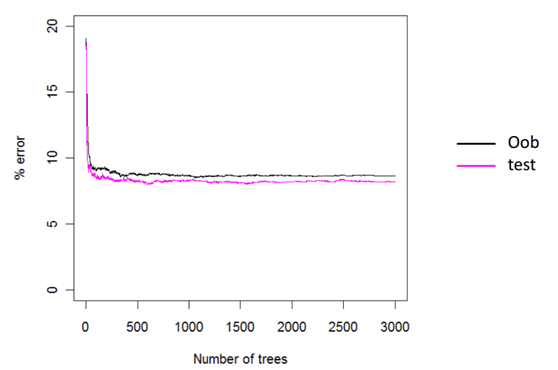
\includegraphics{IMG_2640.png}
\end{center}
Thus, the RF may not look as efficient as KNN after running small dataset. However, as the more and more training data sets put into training, the performance of RF will gradually improved. That's the reason why RF fits for larger scale of dataset, but not the scale like Covtype dataset.
\newline
\newline
In summary, we consider kNN is the best algorithm in dealing with this type
\subsubsection*{Reflection}
\addcontentsline{toc}{subsubsection}{Reflection}
After experiencing the whole process of machine learning, we find that we can do better in the following part:
\newline
\newline
As the description document explained, the dataset contains binary numbers and decimal numbers. With common sense, we should transform the different types of data into unified numbers before training the data set. 
\newline
\newline It seems that the different types of columns did not affect the result too much. Through searching relative researches, we make an explanation that when the data in high dimension space, thus the factor that different types of data will not affect each other or even the training model itself too much.
\newline
\newline
However, what if we do preprocessing with different types of columns separately? If we divide the original dataset into different parts, and how to integrate them again then clustering? We have not research about that.

\section*{Conclusions and Future work}
\addcontentsline{toc}{section}{Conclusions and Future Work}
In conclusion, we choose kNN as the recommended algorithm in dealing with the similar scale of dataset.
\newline
\newline 
Then what can we do in the future? Here are two objectives:
\newline  1.Optimize Random Forest: 
\newline Take Boost algorithm into consideration to optimize the Random Forest method. Try to use Boosting to iterate the data set, and try to modify our new training model based on the last iteration.   
\newline 2.Testing on other algorithms:
\newline Although we have used three methods to analysis this work, we still want to use other methods like SVM, NB to training the data set. Future work will lie on analyzing the advantage of each method to determine a suitable method for this work.   






\newpage



%-------------------------------------------------------------------------------
% REFERENCES
%-------------------------------------------------------------------------------
\newpage
\section*{References}
\addcontentsline{toc}{section}{References}
1. Gama J, Rocha R, Medas P. Accurate decision trees for mining high-speed data streams[C]//Proceedings of the ninth ACM SIGKDD international conference on Knowledge discovery and data mining. ACM, 2003: 523-528.
\newline
\newline
2.Oza N C, Russell S. Experimental comparisons of online and batch versions of bagging and boosting[C]//Proceedings of the seventh ACM SIGKDD international conference on Knowledge discovery and data mining. ACM, 2001: 359-364.
\newline
\newline
3.Obradovic Z, Vucetic S. Challenges in Scientific Data Mining: Heterogeneous, Biased, and Large Samples[R]. Technical Report, Center for Information Science and Technology Temple University, 2004.
\newline
\newline
4.Breiman L. Random forests[J]. Machine learning, 2001, 45(1): 5-32.
\newline
\newline
5.Liaw A, Wiener M. Classification and regression by randomForest[J]. R news, 2002, 2(3): 18-22.

\newpage
\section*{Appendix: How to run}
\addcontentsline{toc}{section}{Appendix: How to run}

1. Generate 10 folds. Run \textit{generate\_samples\_and\_targets.py}. The generated file should be in \textit{data} folder.
\newline
\newline
2. Run Python file for each algorithm. e.g. in command line, run \textit{knn\_with\_orc.py}. The result should be in the \textit{result} folder.

\end{document}


